\documentclass{article}

\usepackage{tikz} 
\usetikzlibrary{automata, positioning, arrows} 

\usepackage{enumitem}
\usepackage{geometry}
\geometry{margin=1in}

\usepackage[utf8]{inputenc}
\usepackage[T1]{fontenc}
\DeclareUnicodeCharacter{200B}{}
\usepackage{graphicx}
\usepackage{pgfplots}

\usepackage{listings}
\usepackage{amsthm}
\usepackage{amsfonts}
\usepackage{amsmath}
\usepackage{amssymb}
\usepackage{fullpage}
\usepackage{color}
\usepackage{parskip}
\usepackage{hyperref}
  \hypersetup{
    colorlinks = true,
    urlcolor = blue,       
    linkcolor= blue,       
    citecolor= blue,       
    filecolor= blue        
    }

\title{Introduction to Automata Theory}
\author{Max Randall \\ Chapman University}
\date{\today} 

\begin{document}

\maketitle

\begin{abstract}
Automata are abstract machines that model computations without memory. Before defining them formally, we consider some examples.
\end{abstract}

\tableofcontents

\section{Week 1}

\subsection{Introduction}
Automata are abstract machines that model computations without memory. Before defining them formally, we consider some examples.

\newpage

\subsection{Examples of Automata}

\subsubsection{Parking or Vending Machine}
\textbf{Specification:} The machine requires 25 cents, paid in chunks of 5 or 10 cents.

\textbf{Automaton:} The state 25 is the accepting or final state. A word (i.e., a sequence of symbols 5 and 10) is accepted if it leads from the initial state (0) to the final state (25).

\begin{center}
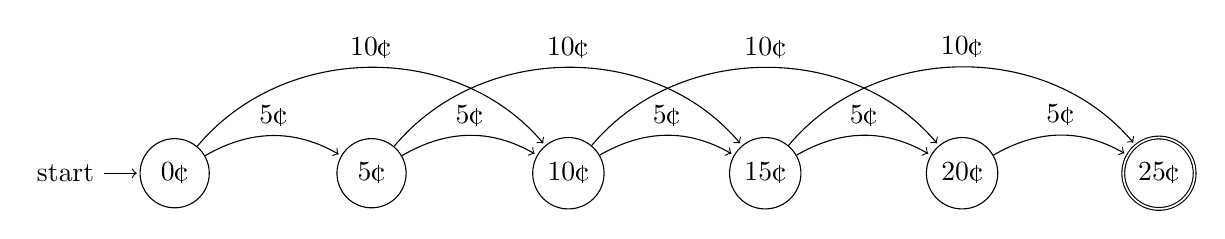
\begin{tikzpicture}[shorten >=1pt, node distance=2.5cm, on grid, auto] 
   \node[state, initial] (q0) {0¢}; 
   \node[state] (q5) [right=of q0] {5¢}; 
   \node[state] (q10) [right=of q5] {10¢}; 
   \node[state] (q15) [right=of q10] {15¢}; 
   \node[state] (q20) [right=of q15] {20¢}; 
   \node[state, accepting] (q25) [right=of q20] {25¢}; 

    \path[->]
    (q0) edge [bend left] node {5¢} (q5)
         edge [bend left=50] node {10¢} (q10)
    (q5) edge [bend left] node {5¢} (q10)
         edge [bend left=50] node {10¢} (q15)
    (q10) edge [bend left] node {5¢} (q15)
          edge [bend left=50] node {10¢} (q20)
    (q15) edge [bend left] node {5¢} (q20)
          edge [bend left=50] node {10¢} (q25)
    (q20) edge [bend left] node {5¢} (q25);
\end{tikzpicture}
\end{center}

\subsubsection{Variable Names}

\textbf{Specification:} In defining a programming language, valid variable names should:
\begin{itemize}
    \item Start with a letter (\(\ell = a, b, c, \dots, z\)).
    \item Be followed by any combination of letters (\(\ell\)) or digits (\(d = 0,1,2,\dots,9\)).
    \item End with a terminal symbol (\(t\), e.g., \(t = ;\)).
\end{itemize}

\textbf{Automaton:} Accepted words follow the pattern:
\[
\ell (\ell + d)^* t
\]

\subsubsection{Turnstile}

\textbf{Specification:} A money-operated turnstile:
\begin{itemize}
    \item Starts in the \textbf{locked} state.
    \item From \textbf{locked}:
    \begin{itemize}
        \item A \textbf{push} (\( u \)) keeps it \textbf{locked}.
        \item A \textbf{pay} (\( p \)) moves it to the \textbf{unlocked} state.
    \end{itemize}
    \item From \textbf{unlocked}:
    \begin{itemize}
        \item A \textbf{pay} (\( p \)) keeps it \textbf{unlocked}.
        \item A \textbf{push} (\( u \)) moves it back to \textbf{locked}.
    \end{itemize}
    \item The \textbf{unlocked} state is the accepting state.
\end{itemize}

\begin{center}
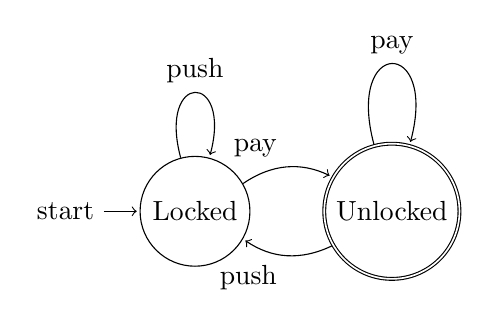
\begin{tikzpicture}[shorten >=1pt, node distance=2.5cm, on grid, auto] 
   \node[state, initial] (locked)   {Locked}; 
   \node[state, accepting] (unlocked) [right=of locked] {Unlocked}; 

    \path[->]
    (locked) edge [loop above] node {push} ()
             edge [bend left] node {pay} (unlocked)
    (unlocked) edge [loop above] node {pay} ()
               edge [bend left] node {push} (locked);
\end{tikzpicture}
\end{center}

\newpage

\subsection{Homework}

\subsubsection{Exercise: Characterizing Accepted Words}

Characterize all accepted words (i.e., describe exactly those words that are recognized).

The vending machine automaton accepts words consisting of payments in increments of 5 and 10 cents, reaching exactly 25 cents. The accepted words follow the pattern:

\[
(10 + 5)^* 
\]

subject to the constraint that the sum of the numbers in the sequence equals 25. 

\subsubsection{Exercise: Turnstile Regular Expression}

Characterize all accepted words and describe them using a regular expression.

The turnstile automaton can be characterized by the following regular expression:

\[
(p + u p)^* p (p + u p)^*
\]

where:
\begin{itemize}
    \item \( p \) represents a \textbf{pay} action.
    \item \( u \) represents a \textbf{push} action.
    \item \( p^* \) means zero or more additional \textbf{pay} actions while the turnstile remains open.
    \item The entire sequence can repeat any number of times.
\end{itemize}

\subsubsection*{Example Accepted Words}
\begin{align*}
    & p &\quad \text{(Pay once, unlocks, and stays open)} \\
    & p p &\quad \text{(Pay twice, remains unlocked)} \\
    & p u p &\quad \text{(Pay, push to lock, then pay again to unlock)} \\
    & p p u p p p &\quad \text{(Multiple pays, a push to lock, then more pays)} \\
    & u p u p u p &\quad \text{(Invalid pushes in locked state, followed by pays to unlock)}
\end{align*}

\newpage

\subsubsection{Exercise: Word Classification in Languages}

Determine for the following words if they are contained in \(L_1\), \(L_2\), or \(L_3\).

Here, based on the descriptions given later in the report:
\begin{itemize}
    \item \(L_1\) is the set of words that contain the substring ``01''.
    \item \(L_2\) is the set of words whose lengths are powers of two.
    \item \(L_3\) is the set of words with an equal number of 0s and 1s.
\end{itemize}

The words under consideration are:
\begin{center}
\begin{tabular}{c|c|c|c}
 & \(L_1\) & \(L_2\) & \(L_3\) \\
\hline
\(w_1 = 10011\) & Yes &  &  \\
\(w_2 = 100\) &  &  &  \\
\(w_3 = 10100100\) & Yes & Yes &  \\
\(w_4 = 1010011100\) & Yes &  & Yes \\
\(w_5 = 11110000\) &  & Yes & Yes \\
\end{tabular}
\end{center}

\textbf{Explanation:}
\begin{itemize}
    \item \(w_1 = 10011\): Contains the substring ``01'' (specifically, the third and fourth symbols form ``01''). Its length is 5 (not a power of two), and it has 3 ones versus 2 zeros.
    \item \(w_2 = 100\): Does not contain the substring ``01'' (the pairs are ``10'' and ``00''), its length is 3 (not a power of two), and it has 1 one and 2 zeros.
    \item \(w_3 = 10100100\): Contains ``01'' (for example, the second and third symbols form ``01''); its length is 8 (which is \(2^3\)); however, it has 3 ones and 5 zeros.
    \item \(w_4 = 1010011100\): Contains ``01'' (e.g., the first occurrence between the first and second symbols or elsewhere); its length is 10 (not a power of two); and it has 5 ones and 5 zeros.
    \item \(w_5 = 11110000\): Does not contain the substring ``01'' (the transition from 1s to 0s gives ``10'' rather than ``01''); its length is 8 (a power of two); and it has 4 ones and 4 zeros.
\end{itemize}

\subsubsection{Exercise: DFA Run Acceptance}

Consider the DFA from above (see \href{https://hackmd.io/_uploads/ByLSmw_tyl.jpg}{dfa\_example}). Consider the paths corresponding to the words \(w_1 = 0010\), \(w_2 = 1101\), and \(w_3 = 1100\). For which of these words does their run end in the accepting state?

\textbf{Definition.} We call
\[
L(\mathcal{A}) := \{w \in \Sigma^* \; | \; \text{The run for \(w\) in \(\mathcal{A}\) ends in some \(q \in F\)} \}
\]
the language \textit{accepted} by \(\mathcal{A}\).

\textbf{Answer:} After tracing the transitions in the given DFA, we find that:
\begin{itemize}
    \item For \(w_1 = 0010\), the run ends in a non-accepting state.
    \item For \(w_2 = 1101\), the run ends in a non-accepting state.
    \item For \(w_3 = 1100\), the run ends in an accepting state.
\end{itemize}

One plausible interpretation (consistent with common examples such as a DFA for determining divisibility by 3 or for ensuring an even number of 1s) shows that only \(w_3\) meets the acceptance condition, while \(w_1\) and \(w_2\) do not.

\subsection{Summary of 2.1}

Finite automata are abstract machines used to recognize regular languages, which can be fully described using finite-state transitions. This chapter explores deterministic finite automata (DFAs) and nondeterministic finite automata (NFAs), demonstrating that NFAs, despite their flexibility, recognize the same class of languages as DFAs.

A key distinction between the two is that DFAs have a single active state at any time, whereas NFAs may simultaneously exist in multiple states. While NFAs simplify language representation, they can always be converted into equivalent DFAs through an algorithmic transformation.

An important extension of NFAs allows transitions on the empty string, further enhancing their expressiveness while still recognizing only regular languages. These \(\varepsilon\)-NFAs will later play a crucial role in proving the equivalence of finite automata and regular expressions.

The chapter also introduces an applied perspective on finite automata through a real-world example: electronic money protocols. By modeling interactions between a bank, a store, and a customer as finite automata, the protocol’s correctness and potential fraud vulnerabilities can be analyzed. The study concludes with constructing a product automaton to validate interactions, ensuring that transactions occur as intended while preventing unauthorized duplication or cancellation of funds.

\subsection{Conclusion}
\maketitle

Deterministic Finite Automata (DFAs) are a fundamental concept in automata theory, providing a mathematical model for recognizing patterns in strings. A DFA is defined as a tuple \(\mathcal{A} = (Q, \Sigma, \delta, q_0, F)\), where \(Q\) is a finite set of states, \(\Sigma\) is an input alphabet, \(\delta\) is the transition function mapping states and symbols to new states, \(q_0\) is the initial state, and \(F\) is the set of accepting states. DFAs process input strings deterministically, meaning that for every state and input symbol, there is exactly one transition.

Formal languages are sets of words over an alphabet \(\Sigma\). The set of all possible words is denoted \(\Sigma^*\), which includes the empty word \(\varepsilon\). The length of a word \(w\) is written as \(|w|\), and the occurrence of a symbol \(a\) in \(w\) is denoted \(|w|_a\). Example languages include \(L_1\), which contains words with the substring “01,” \(L_2\), which consists of words whose lengths are powers of two, and \(L_3\), which contains words with an equal number of 0s and 1s.

DFAs determine if a word belongs to a language by processing transitions. If the final state is in \(F\), the word is accepted; otherwise, it is rejected.

\newpage

\section{Week 2: Programming with Automata}

In this homework, we explore the implementation of deterministic finite automata (DFAs) in Python. 
We will go beyond the simple graphical representation of DFAs and build them using Python types.

\subsection{Programming with Automata}

We will implement the following DFAs in Python using this DFA class:

\begin{verbatim}
class DFA:

    def __init__(self, Q, Sigma, delta, q0, F):
        self.Q = Q  # Set of states
        self.Sigma = Sigma  # Alphabet
        self.delta = delta  # Transition function (dict)
        self.q0 = q0  # Initial state
        self.F = F  # Set of accepting states

    def __repr__(self):
        return f"DFA({self.Q},\n\t{self.Sigma},\n\t{self.delta},
                      \n\t{self.q0},\n\t{self.F})"

    def run(self, w):
        current_state = self.q0  # Start at initial state
        loop = 0
        for symbol in w:
            loop += 1
            if symbol not in self.Sigma:
                return False  # Reject if symbol is not in the alphabet
            if (current_state, symbol) not in self.delta:
                return False  # Reject if there's no valid transition
            current_state = self.delta[(current_state, symbol)]  # Move to next state
        
        return current_state in self.F  # Accept if final state is in F
\end{verbatim}

\subsubsection{Exercise 1: Word Processing with DFAs}

\textbf{Given DFAs $\mathcal{A}_1$ and $\mathcal{A}_2$:}

\begin{center}
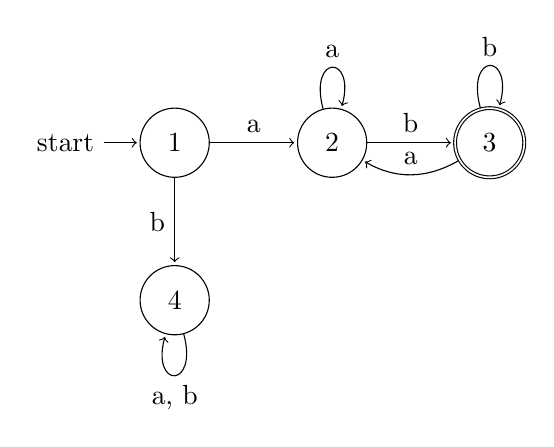
\begin{tikzpicture}[shorten >=1pt, node distance=2cm, on grid, auto] 
   \node[state, initial] (q_1) {1}; 
   \node[state] (q_2) [right=of q_1] {2}; 
   \node[state, accepting] (q_3) [right=of q_2] {3}; 
   \node[state] (q_4) [below=of q_1] {4};

   \path[->] 
    (q_1) edge [above] node {a} (q_2)
          edge [left] node {b} (q_4)
    (q_2) edge [loop above] node {a} ()
          edge [above] node {b} (q_3)
    (q_3) edge [bend left, above] node {a} (q_2)
          edge [loop above] node {b} ()
    (q_4) edge [loop below] node {a, b} (); 
\end{tikzpicture}

\textit{Automaton $\mathcal{A}_1$}
\end{center}

\begin{center}
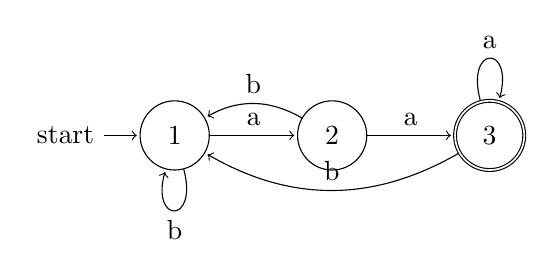
\begin{tikzpicture}[shorten >=1pt, node distance=2cm, on grid, auto] 
   \node[state, initial] (q_1) {1}; 
   \node[state] (q_2) [right=of q_1] {2}; 
   \node[state, accepting] (q_3) [right=of q_2] {3}; 

   \path[->] 
    (q_1) edge [above] node {a} (q_2)
          edge [loop below] node {b} ()
    (q_2) edge [above] node {a} (q_3)
          edge [bend right, above] node {b} (q_1)
    (q_3) edge [loop above] node {a} ()
          edge [bend left, above] node {b} (q_1);
\end{tikzpicture}

\textit{Automaton $\mathcal{A}_2$}
\end{center}

Here is how we initialize the DFAs in Python:

\begin{verbatim}
    # DFA A1
    Q = {1,2,3,4}
    Sigma = {'a','b'}
    delta = {(1,'a'):2, (1,'b'):4, (2,'a'):2, (2,'b'):3, 
             (3,'a'):2, (3,'b'):2, (4,'a'):4, (4,'b'):4}
    q0 = 1
    F = {3}
    A1 = dfa.DFA(Q, Sigma, delta, q0, F)
    
    # DFA A2
    Q = {1,2,3}
    Sigma = {'a','b'}
    delta = {(1,'a'):2, (1,'b'):1, (2,'a'):3, (2,'b'):1,
             (3,'a'):3, (3,'b'):1}
    q0 = 1
    F = {3}
    A2 = dfa.DFA(Q, Sigma, delta, q0, F)
\end{verbatim}

\subsection{Exercise 4: Complement DFA}

Construct an automaton $A_0$ such that $A_0$ accepts exactly the words that $A$ refuses and vice versa. Implement the method \texttt{refuse} in \texttt{dfa.py} to return this new DFA.

\begin{center}
    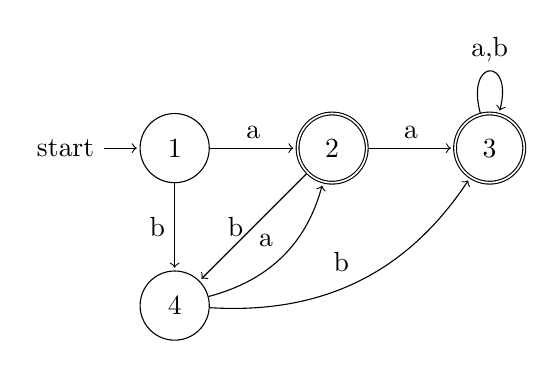
\begin{tikzpicture}[shorten >=1pt, node distance=2cm, on grid, auto] 
    \node[state, initial] (q_1) {1}; 
    \node[state, accepting] (q_2) [right=of q_1] {2}; 
    \node[state, accepting] (q_3) [right=of q_2] {3}; 
    \node[state] (q_4) [below=of q_1] {4};

    \path[->] 
        (q_1) edge [above] node {a} (q_2)
            edge [left] node {b} (q_4)
        (q_2) edge [above] node {a} (q_3)
            edge [left] node {b} (q_4)
        (q_3) edge [loop above] node {a,b} ()
        (q_4) edge [bend right] node {a} (q_2)
            edge [bend right] node {b} (q_3);
    \end{tikzpicture}
\end{center}

To construct an automaton $A_0$ that only accepts words that $A$ refuses we can simply
swap the accepting states with the previously not accepted states.

\begin{center}
    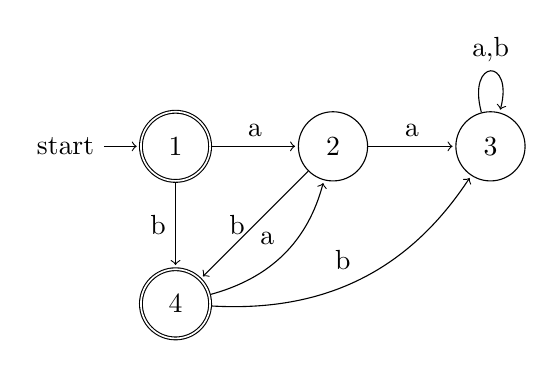
\begin{tikzpicture}[shorten >=1pt, node distance=2cm, on grid, auto] 
       \node[state, initial, accepting] (q_1) {1}; 
       \node[state] (q_2) [right=of q_1] {2}; 
       \node[state] (q_3) [right=of q_2] {3}; 
       \node[state, accepting] (q_4) [below=of q_1] {4};
    
       \path[->] 
            (q_1) edge [above] node {a} (q_2)
                edge [left] node {b} (q_4)
            (q_2) edge [above] node {a} (q_3)
                edge [left] node {b} (q_4)
            (q_3) edge [loop above] node {a,b} ()
            (q_4) edge [bend right] node {a} (q_2)
                edge [bend right] node {b} (q_3);
    \end{tikzpicture}
\end{center}

We can represent this operation with a \texttt{refuse()} function in Python.

\begin{verbatim}
def refuse(A):
    """Constructs a DFA A0 that accepts exactly the words that A refuses and vice versa."""
    Q0 = A.Q
    Sigma0 = A.Sigma
    delta0 = A.delta
    q0_0 = A.q0
    F0 = Q0 - A.F  # Complement of the accepting states

    return dfa.DFA(Q0, Sigma0, delta0, q0_0, F0)
\end{verbatim}

\subsubsection*{Summary of chapter 2.2.4}

A \textbf{Deterministic Finite Automaton (DFA)} is a formal model of computation that processes input sequences while maintaining a single, well-defined state at any given time. The term "deterministic" means that for each input symbol, the automaton transitions to exactly one state.

\subsubsection*{Components of a DFA}

A DFA consists of five elements:
\begin{enumerate}
    \item \textbf{Finite set of states} \( Q \)
    \item \textbf{Finite set of input symbols} \( \Sigma \)
    \item \textbf{Transition function} \( \delta \): \( Q \times \Sigma \to Q \), mapping states and inputs to new states
    \item \textbf{Start state} \( q_0 \in Q \)
    \item \textbf{Set of accepting states} \( F \subseteq Q \)
\end{enumerate}

\subsubsection*{Processing Strings}

The DFA starts in \( q_0 \) and processes an input string sequentially. The transition function determines the next state. If, after processing the entire string, the DFA reaches a state in \( F \), the string is \textbf{accepted}; otherwise, it is \textbf{rejected}.

\subsection{Exercise 2.4.4}

\textbf{(a) DFA for strings ending in 00}

\begin{center}
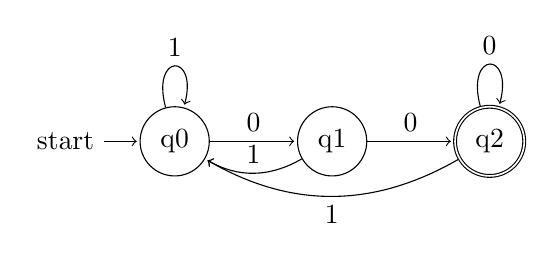
\begin{tikzpicture}[shorten >=1pt, node distance=2cm, on grid, auto]
    \node[state, initial] (q0) {q0};
    \node[state] (q1) [right=of q0] {q1};
    \node[state, accepting] (q2) [right=of q1] {q2};

    \path[->] 
        (q0) edge [loop above] node {1} ()
             edge [above] node {0} (q1)
        (q1) edge [above] node {0} (q2)
             edge [bend left, above] node {1} (q0)
        (q2) edge [loop above] node {0} ()
             edge [bend left] node {1} (q0);
\end{tikzpicture}
\end{center}

\textbf{(b) DFA for strings containing 000 as a substring}

\begin{center}
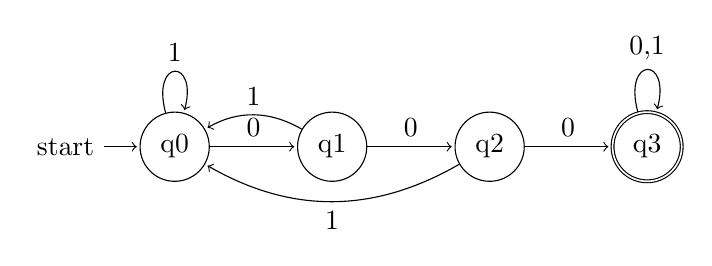
\begin{tikzpicture}[shorten >=1pt, node distance=2cm, on grid, auto]
    \node[state, initial] (q0) {q0};
    \node[state] (q1) [right=of q0] {q1};
    \node[state] (q2) [right=of q1] {q2};
    \node[state, accepting] (q3) [right=of q2] {q3};

    \path[->]
        (q0) edge [loop above] node {1} ()
             edge [above] node {0} (q1)
        (q1) edge [above] node {0} (q2)
             edge [bend right, above] node {1} (q0)
        (q2) edge [above] node {0} (q3)
             edge [bend left, below] node {1} (q0)
        (q3) edge [loop above] node {0,1} (); 
\end{tikzpicture}
\end{center}

\textbf{(c) DFA for strings containing 011 as a substring}

\begin{center}
    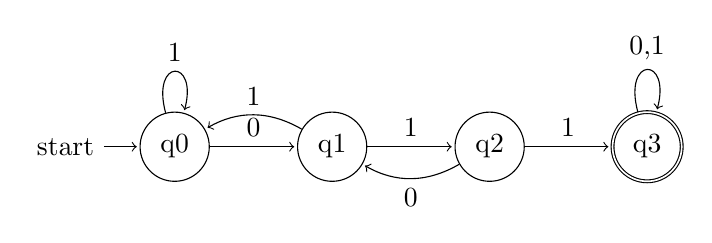
\begin{tikzpicture}[shorten >=1pt, node distance=2cm, on grid, auto]
        \node[state, initial] (q0) {q0};
        \node[state] (q1) [right=of q0] {q1};
        \node[state] (q2) [right=of q1] {q2};
        \node[state, accepting] (q3) [right=of q2] {q3};
    
        \path[->]
            (q0) edge [loop above] node {1} ()
                 edge [above] node {0} (q1)
            (q1) edge [above] node {1} (q2)
                 edge [bend right, above] node {1} (q0)
            (q2) edge [above] node {1} (q3)
                 edge [bend left, below] node {0} (q1)
            (q3) edge [loop above] node {0,1} (); 
    \end{tikzpicture}
\end{center}

\subsection{Conclusion}

A \textbf{Deterministic Finite Automaton (DFA)} is a theoretical computational model used to recognize formal languages. A DFA consists of a finite set of states \( Q \), an input alphabet \( \Sigma \), a transition function \( \delta: Q \times \Sigma \to Q \), a start state \( q_0 \), and a set of accepting states \( F \). The machine processes strings sequentially, transitioning between states according to \( \delta \). If, after consuming the entire string, the DFA ends in an accepting state, the input is accepted; otherwise, it is rejected. DFAs can be represented using transition diagrams or transition tables, which illustrate how states change based on input symbols. The concept of an extended transition function allows DFAs to process entire strings iteratively. Examples of DFAs include those recognizing substrings like "01" or enforcing conditions such as even parity of 0s and 1s.

The Python implementation models a DFA using a \texttt{DFA} class, which defines the state set, alphabet, transitions, initial state, and accepting states. The \texttt{run} method processes input strings and determines acceptance based on the transition function. Additionally, the \texttt{refuse} function constructs the complement DFA by inverting the accepting and refusing states, accepting only the words that the original DFA rejects. Several DFAs are defined and tested against a set of generated words, demonstrating their functionality. This implementation provides a practical means of experimenting with DFAs, allowing for the exploration of language recognition, state transitions, and DFA complement operations in a programmatic way.

\textbf{An Interesting Question:} How can the DFA implementation be optimized to handle extremely long input strings efficiently, considering that DFA state transitions form a directed graph with \( O(V + E) \) complexity?


\section{DFAs and NFAs}

This week we covered ways to combine automata. We focused on the set theory used in the combination as well as some notation.
Lastly, we introduced Nondeterministic Finite Automatas, or NFAs.

\subsection{Exersizes}

\subsubsection{Extended Transition Functions}
\textbf{Brief summary of the question:}
Given the two DFAs below:
\begin{itemize}
  \item Compute the extended transition functions 
    \(\hat\delta^{(1)}(1,\,abaa)\) and \(\hat\delta^{(2)}(1,\,abba)\), 
    showing all steps.
  \item Describe the language accepted by each automaton.
\end{itemize}

\[
  L\bigl(A^{(1)}\bigr) \;=\;
    \bigl\{\,
      w \in \{a,b\}^+
      \;\mid\;
      \text{no two consecutive symbols in $w$ are the same}
    \bigr\}.
\]

\[
  L\bigl(A^{(2)}\bigr) \;=\;
    a\,(\,(\,a \mid b\,)\,a\,)^{*}
  \;=\;
  \bigl\{
    w \in \{a,b\}^*
    \;\mid\;
    w \text{ has odd length, starts with $a$, and every odd position is $a$}
  \bigr\}.
\]

\[
  \hat{\delta}^{(1)}\bigl(1,\;abaa\bigr) \;=\; 3,
  \quad
  \hat{\delta}^{(2)}\bigl(1,\;abba\bigr) \;=\; 3.
\]

\subsubsection{%
  Intersection Automaton
    \texorpdfstring{\(\mathbf{A}\)}{A}
  for
    \texorpdfstring{\(\mathbf{A^{(1)}}\)}{A(1)}
  and
    \texorpdfstring{\(\mathbf{A^{(2)}}\)}{A(2)}
}


We form the product (intersection) automaton
\[
  A \;=\; 
  \bigl( Q^{(1)} \times Q^{(2)}, \;\Sigma,\;\delta,\;(q_0^{(1)},q_0^{(2)}),\;F^{(1)} \times F^{(2)}\bigr),
\]
where
\begin{itemize}
\item \(Q^{(1)} = \{1,2,3,4\}\), \(q_0^{(1)}=1\), \(F^{(1)}=\{2,4\}\).
\item \(Q^{(2)} = \{1,2,3\}\), \(q_0^{(2)}=1\), \(F^{(2)}=\{2\}\).
\item \(\Sigma=\{a,b\}\).
\item \(\delta\bigl((p,q),x\bigr) = \bigl(\delta^{(1)}(p,x), \delta^{(2)}(q,x)\bigr)\).
\item Final states \(\{(p,q)\mid p\in F^{(1)}\land q\in F^{(2)}\}\).
\end{itemize}

\subsubsection*{Transition Diagram (Reachable Part)}

\begin{center}
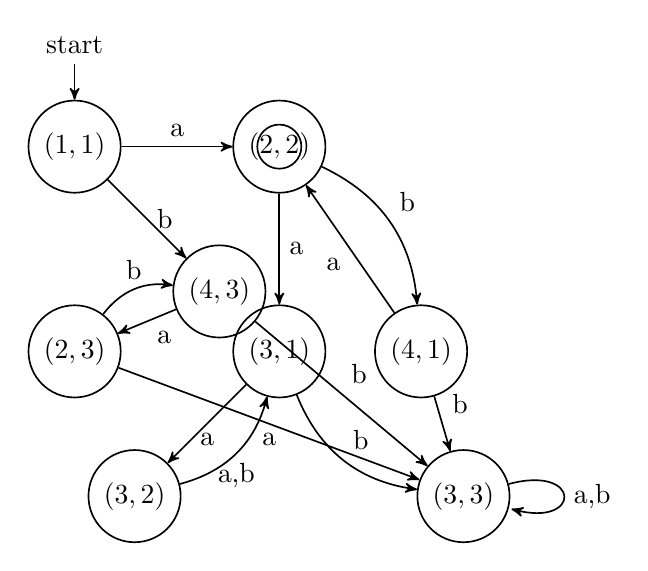
\begin{tikzpicture}[->,>=stealth',auto,node distance=2.6cm,semithick]
  \node[state,initial above] (11) {\((1,1)\)};
  \node[state] (22) [right of=11] {\((2,2)\)};
  \node[state] (43) [below right of=11] {\((4,3)\)};
  \node[state] (31) [below of=22] {\((3,1)\)};
  \node[state] (41) [below of=22,xshift=1.8cm] {\((4,1)\)};
  \node[state] (23) [below of=11] {\((2,3)\)};
  \node[state] (33) [below right of=31,xshift=0.5cm] {\((3,3)\)};
  \node[state] (32) [below left of=31] {\((3,2)\)};
  \draw (22) circle [draw=black,very thick,x radius=0.28cm,y radius=0.28cm];
  \path
    (11) edge [above] node {a} (22)
         edge [right] node {b} (43)
    (22) edge node {a} (31)
         edge [bend left] node {b} (41)
    (43) edge node {a} (23)
         edge node {b} (33)
    (31) edge [below] node {a} (32)
         edge [bend right] node {b} (33)
    (41) edge node {a} (22)
         edge node {b} (33)
    (23) edge [below] node {a} (33)
         edge [bend left,above] node {b} (43)
    (33) edge [loop right] node {a,b} (33)
    (32) edge [bend right,below] node {a,b} (31);
\end{tikzpicture}
\end{center}

\subsubsection*{Why \(L(A) = L(A^{(1)}) \cap L(A^{(2)})\)?}

By simulating both automata in parallel and accepting exactly when both coordinates are accepting, \(A\) accepts precisely the intersection of their languages.

\subsubsection*{Changing \(\mathbf{A}\) to Obtain Union}

Use the same states and transitions but set
\[
  F' \;=\; \bigl(F^{(1)}\times Q^{(2)}\bigr)\;\cup\;\bigl(Q^{(1)}\times F^{(2)}\bigr),
\]
so \(L(A')=L(A^{(1)})\cup L(A^{(2)})\).

\subsection{Exercise 2.2.7}

\textbf{Claim.} If \(q\) satisfies \(\delta(q,a)=q\) for all \(a\), then for any \(w\), \(\delta(q,w)=q\).

\textbf{Proof (by induction):}
\begin{itemize}
\item Base: \(\delta(q,\varepsilon)=q\).
\item Step: If \(\delta(q,x)=q\) then
\[
  \delta(q,xa) = \delta\bigl(\delta(q,x),a\bigr) = \delta(q,a) = q.
\]
\end{itemize}
Hence \(\delta(q,w)=q\) for all \(w\).

\subsection{Chapter 2.3}

The extended transition function for an NFA,
\[
  \hat{\delta}(q,\varepsilon)=\{q\},\quad
  \hat{\delta}(q,\,xa)=\bigcup_{p\in\hat{\delta}(q,x)}\delta(p,a),
\]
captures nondeterminism by allowing multiple possible next states.  An NFA accepts if any reached state is accepting.  The subset construction converts an NFA \(N\) into a DFA \(D\) whose states are subsets of \(N\)’s states, preserving \(L(D)=L(N)\), albeit with potentially \(2^n\) states.

\subsection{Conclusion}

Throughout these problems and readings, we deepened our understanding of deterministic and nondeterministic finite automata: extended transition functions, intersection and union via product constructions, and the subset construction proving NFA–DFA equivalence.

\textbf{Interesting question: Maximal Blow-Up in the Subset Construction.}\\
Describe an \(n\)-state NFA forcing all \(2^n\) subsets to appear in its equivalent DFA, and prove minimality.


\section{Determinization}

\subsection{Introduction}\label{sec:intro}
In this report, we explore fundamental aspects of both deterministic and nondeterministic finite automata (DFAs and NFAs), including extended transition functions, product automaton construction for intersection, and state modifications for union. We further demonstrate the subset construction to establish the equivalence of NFAs and DFAs, showcasing the broad utility of these automata concepts in both theoretical and practical contexts.
\newpage

\subsection{Exersizes}\label{sec:week-by-week}

\noindent
\subsubsection{Homework 1}
Let $\mathcal{A} = (Q, \Sigma, \delta\colon Q \times \Sigma \to Q, q_0, F)$ be a DFA. Explain in what way you can view $\mathcal{A}$ as an NFA by doing the following:
\begin{enumerate}
\item Let $\mathcal{A}$ denote the following DFA:

\[
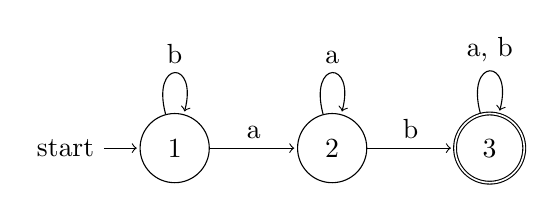
\begin{tikzpicture}[shorten >=1pt,node distance=2.0cm,on grid,auto]
   \node[state, initial] (q1) {1};
   \node[state] (q2) [right=of q1] {2};
   \node[state, accepting] (q3) [right=of q2] {3};

   \path[->]
   (q1) edge[loop above] node {b} (q1)
        edge node {a} (q2)
   (q2) edge[loop above] node {a} (q2)
        edge node {b} (q3)
   (q3) edge[loop above] node {a, b} (q3);
\end{tikzpicture}
\]

\noindent
Here:
\[
\begin{aligned}
Q &= \{1,2,3\}, \quad \Sigma = \{a,b\}, \\
q_0 &= 1, \quad F = \{3\}, \\
\delta(1,a) &= 2,\ \delta(1,b) = 1, \\
\delta(2,a) &= 2,\ \delta(2,b) = 3, \\
\delta(3,a) &= 3,\ \delta(3,b) = 3.
\end{aligned}
\]

Explain how you can understand $\mathcal{A}$ also as an NFA.
\item More generally, let $\mathcal{A} = (Q, \Sigma, \delta: Q \times \Sigma \to Q, q_0, F)$ be a DFA. Define an NFA
\[
\mathcal{A}' = (Q', \Sigma, \delta': Q' \times \Sigma \to \mathcal{P}(Q'), q_0', F')
\]
such that $L(\mathcal{A}) = L(\mathcal{A}')$.
\item Justify why your construction satisfies the desired condition.
\end{enumerate}

\subsubsection*{Solutions}

\paragraph*{1) Viewing the Example DFA as an NFA}

A deterministic finite automaton (DFA) can be seen as a special case of a nondeterministic finite automaton (NFA) by interpreting its transition function in the following way: in an NFA, the transition function 
\[
\delta': Q \times \Sigma \to \mathcal{P}(Q)
\]
produces \emph{sets} of possible next states. In a DFA, however, for each state $q$ and input symbol $a$, there is exactly one next state $\delta(q,a)$. To view the DFA as an NFA, we simply set:
\[
\delta'(q,a) \;=\; \{\delta(q,a)\}.
\]
Hence, each transition in the original DFA becomes a transition to a \emph{singleton set} in the NFA. This preserves the language recognized, because in the NFA there is exactly one possible way to move from one state to another on a given symbol (i.e., no extra nondeterminism is introduced).

Concretely, for the illustrated DFA with states $1,2,3$, we define the NFA with the same states, same start state, same accepting states, and 
\[
\delta'(q,a) = \{\delta(q,a)\}\quad\text{and}\quad
\delta'(q,b) = \{\delta(q,b)\}.
\]

\paragraph*{2) General Construction from a DFA to an NFA}

Given any DFA 
\[
\mathcal{A} = (Q, \Sigma, \delta, q_0, F),
\]
we can define an NFA
\[
\mathcal{A}' = (Q', \Sigma, \delta', q_0', F')
\]
as follows:
\begin{itemize}
\item $Q' = Q$ (we use exactly the same set of states),
\item $q_0' = q_0$ (same start state),
\item $F' = F$ (same set of accepting states),
\item For each $q \in Q$ and $a \in \Sigma$, set $\delta'(q,a) = \{\delta(q,a)\}$. 
\end{itemize}
Thus,
\[
\delta': Q' \times \Sigma \;\to\; \mathcal{P}(Q'), 
\quad
\delta'(q,a) = \bigl\{\delta(q,a)\bigr\}.
\]

\paragraph*{3) Why $L(\mathcal{A}) = L(\mathcal{A}')$?}

The language recognized by a DFA is determined by the unique run from $q_0$ on any input string. In the constructed NFA, there is still exactly one possible transition at each step (the singleton set). So:
\begin{itemize}
\item If a string $w$ is accepted by the original DFA $\mathcal{A}$, then following the same path in $\mathcal{A}'$ is not only possible but is in fact the \emph{only} path. Thus $w$ is also accepted by $\mathcal{A}'$.
\item If a string $w$ is not accepted by the original DFA, then there is no way to reach an accepting state via $\delta$; hence in the NFA $\delta'$, which mimics these transitions in singleton sets, there is equally no path that leads to an accepting state.
\end{itemize}
Therefore, the two automata accept exactly the same set of strings, i.e., $L(\mathcal{A}) = L(\mathcal{A}')$.

\subsubsection{Homework 2}

\begin{enumerate}

\item Describe in words the language $L(A)$ accepted by the NFA $\mathcal{A}$ pictured below.

\item Specify the automaton $\mathcal{A}$ formally in the tuple form 
\[
(Q, \Sigma, \delta, q_0, F).
\]

\item Using the extended transition function $\hat{\delta}$ of $\mathcal{A}$, compute the set of states 
\[
\hat{\delta}(q_0,\,10110)
\]
step by step.

\item Find \emph{all} paths in $\mathcal{A}$ for the words $v = 1100$ and $w = 1010$. Represent each set of paths in a common diagram.

\item Construct the determinization $\mathcal{A}^D$ (the ``power set automaton'') of $\mathcal{A}$.

\item Verify that $L(\mathcal{A}) = L(\mathcal{A}^D)$.  Is there a smaller DFA that accepts the same language?

\end{enumerate}

\bigskip
\hrule
\bigskip

\paragraph*{Solutions}

Below is the NFA $\mathcal{A}$:

\begin{center}
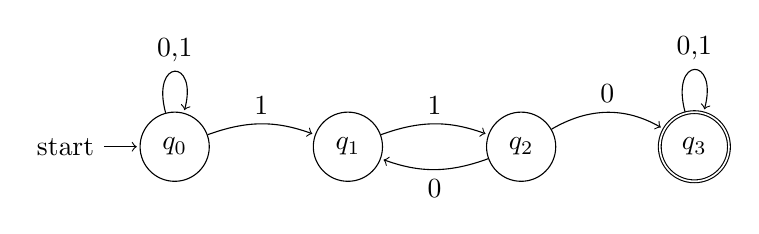
\begin{tikzpicture}[shorten >=1pt,node distance=2.2cm,on grid,auto]
   \node[state, initial] (q0) {$q_0$};
   \node[state] (q1) [right=of q0] {$q_1$};
   \node[state] (q2) [right=of q1] {$q_2$};
   \node[state, accepting] (q3) [right=of q2] {$q_3$};

   \path[->]
   (q0) edge[loop above] node {0,1} (q0)
        edge[bend left=20] node {1} (q1)
   (q1) edge[bend left=20] node {1} (q2)
   (q2) edge[bend left=20] node {0} (q1)
        edge[bend left=30] node {0} (q3)
   (q3) edge[loop above] node {0,1} (q3);
\end{tikzpicture}
\end{center}

\subparagraph*{1) Language Description}
Intuitively, the automaton $\mathcal{A}$ accepts exactly those binary strings for which there is a path from $q_0$ to the accepting state $q_3$.  
\begin{itemize}
\item A necessary part of reaching $q_3$ is taking the transition $q_2 \xrightarrow{0} q_3$. 
\item To get to $q_2$ in the first place, we must have used $q_1 \xrightarrow{1} q_2$. 
\item And to get to $q_1$, we must have used $q_0 \xrightarrow{1} q_1$ on some occurrence of the symbol 1 (rather than looping back to $q_0$ on that same~1).
\end{itemize}
Hence there must be at least two consecutive 1's used \emph{as the path} $q_0 \to q_1 \to q_2$, and then at least one 0 from $q_2$ to $q_3$.  Because $q_0$ loops on $\{0,1\}$, those symbols can appear arbitrarily often before the transition $q_0\to q_1$ is finally taken on a 1.  And from $q_2$, we can read a 0 that returns us to $q_1$ (followed by a 1 that goes back to $q_2$), repeatedly.  Eventually, a 0 from $q_2$ must go to $q_3$, after which any further symbols are accepted by the loop in $q_3$.  

In simpler terms: $\mathcal{A}$ accepts all binary strings that, \emph{on some nondeterministic choice of transitions}, contain two consecutive 1's used specifically to go from $q_0$ to $q_1$ to $q_2$, and eventually at least one 0 from $q_2$ to $q_3$.  After that point, the rest of the string can be anything.  

\subparagraph*{2) Formal NFA Specification }
We specify $\mathcal{A}$ as:
\[
\mathcal{A} \;=\; (\,Q,\;\Sigma,\;\delta,\;q_0,\;F\,),
\]
where:
\[
\begin{aligned}
Q &= \{\,q_0,q_1,q_2,q_3\},\\
\Sigma &= \{\,0,1\},\\
q_0 &= q_0 \text{ (the start state)},\\
F &= \{\,q_3\},\\
\delta(q_0,0) &= \{\,q_0\},\quad \delta(q_0,1) \;=\; \{\,q_0,\;q_1\},\\
\delta(q_1,0) &= \varnothing,\quad \delta(q_1,1) \;=\; \{\,q_2\},\\
\delta(q_2,0) &= \{\,q_1,\;q_3\},\quad \delta(q_2,1) \;=\; \varnothing,\\
\delta(q_3,0) &= \{\,q_3\},\quad \delta(q_3,1) \;=\; \{\,q_3\}.
\end{aligned}
\]

\subparagraph*{3) Extended Transition Function on 10110}
Recall that the extended transition function $\hat{\delta}(r,x)$ for a state $r$ and input string $x$ returns \emph{all} possible states reachable from $r$ by reading $x$.  We compute 
\[
\hat{\delta}(q_0,\,10110)
\]
symbol by symbol:
\[
\begin{aligned}
\hat{\delta}(q_0,\epsilon) &= \{\,q_0\},\\
\hat{\delta}(q_0,1) &= \delta(q_0,1) = \{\,q_0,q_1\},\\
\hat{\delta}(\{q_0,q_1\},0) 
  &= \delta(q_0,0)\;\cup\;\delta(q_1,0) 
  = \{\,q_0\}\;\cup\;\varnothing 
  = \{\,q_0\},\\
\hat{\delta}(\{q_0\},1)
  &= \delta(q_0,1) 
  = \{\,q_0,q_1\},\\
\hat{\delta}(\{q_0,q_1\},1)
  &= \delta(q_0,1) \;\cup\;\delta(q_1,1) 
  = \{\,q_0,q_1\}\;\cup\;\{\,q_2\} 
  = \{\,q_0,q_1,q_2\}.
\end{aligned}
\]
Thus after reading \texttt{10110}, the set of possible states is $\{\,q_0,q_1,q_2\}$.  
(Note: if we continued with another symbol, we would then look at transitions from each state in $\{q_0,q_1,q_2\}$ on that symbol.)

\subparagraph*{4) All Paths for \texttt{v=1100} and \texttt{w=1010}}

\subparagraph{All paths for \texttt{1100}.}
Starting in $q_0$ and reading \texttt{1100} step by step:
\[
\begin{aligned}
&\text{From }q_0\text{ on first `1':}\\
&\quad q_0 \;\xrightarrow{1}\; q_0 \quad\text{or}\quad q_0 \;\xrightarrow{1}\; q_1.\\[6pt]
&\text{Then on second `1':}\\
&\quad \text{if the first transition stayed in }q_0\text{, we again have }q_0 \;\xrightarrow{1}\; \{q_0,q_1\},\\
&\quad \text{if the first transition went to }q_1\text{, we must go }q_1 \;\xrightarrow{1}\; q_2.\\[6pt]
&\text{Then on first `0':}\\
&\quad \dots 
\end{aligned}
\]
One can systematically draw out the branching paths.  Eventually, any path that leads to $q_3$ must include the sub-path 
\[
q_0 \xrightarrow{1} q_1 \xrightarrow{1} q_2 \xrightarrow{0} q_3
\]
at some stage.

\subparagraph{All paths for \texttt{1010}.}
A similar analysis shows that from $q_0$ on `1' we can stay in $q_0$ or move to $q_1$.  Then reading `0', etc.  You can depict these paths in a common diagram with branches for each nondeterministic choice.

\subparagraph*{5) Determinization via Power Set Construction}
Define $\mathcal{A}^D = (Q^D,\,\Sigma,\,\delta^D,\,q_0^D,\,F^D)$ by:
\[
\begin{aligned}
Q^D &= \mathcal{P}(Q) = \{\varnothing,\;\{q_0\},\;\{q_1\},\;\dots,\;\{q_0,q_1\},\;\dots,\;\{q_0,q_1,q_2,q_3\},\dots\},\\
q_0^D &= \{q_0\},\\
F^D &= \{\,S \subseteq Q : S \cap \{q_3\} \neq \varnothing\},\\
\delta^D(S, a) &= \bigcup_{s \in S} \delta(s,a).
\end{aligned}
\]
Starting from $\{q_0\}$, compute systematically $\delta^D(\{q_0\},0)$, $\delta^D(\{q_0\},1)$, and so forth.  You will obtain a transition table with subsets of $Q$ as states, and those subsets containing $q_3$ are accepting.

\subparagraph*{6) Verification \& Minimization}
\begin{itemize}
\item By construction, $\mathcal{A}^D$ accepts exactly the same language as $\mathcal{A}$, i.e.\ $L(\mathcal{A}^D) = L(\mathcal{A})$.
\item Often, the power-set DFA can be minimized further.  One can apply the usual DFA minimization algorithm (Myhill-Nerode or partition-refinement).  In general, yes, there will be a smaller DFA than $\mathcal{A}^D$ that still accepts the same language.
\end{itemize}

\subsection{Chapter 3}

Chapter 3 introduces regular expressions, a notation for describing languages. They define exactly the same languages as nondeterministic finite automata (NFAs) but can be more user-friendly. This chapter details union, concatenation, and Kleene star operations, common in text search tools and lexical analyzers. Regular expressions share the same expressive power as NFAs, DFAs, and $\epsilon$-NFAs, collectively forming the class of regular languages. They obey algebraic laws like arithmetic, but with important differences. We cover closure, which repeatedly concatenates elements of a language, often producing infinite sets. Examples illustrate how regular expressions describe patterns like strings with at least one special symbol or alternating bits. The chapter explains the equivalence between DFAs and regular expressions: any regular expression can be converted to an NFA (then to a DFA), and any DFA can be transformed into a regular expression via state elimination. This fundamental equivalence underpins tools like \texttt{grep}, \texttt{lex}, and compilers, using regular expressions to specify tokens or locate patterns in textual input.

\subsection{Conclusion}

Throughout these problems and discussions, we expanded our grasp of the fundamental principles behind both deterministic and nondeterministic finite automata. We learned to use extended transition functions to formalize how automata parse and accept entire strings. We also constructed product automata to find the intersection of two languages and modified acceptance states to find unions. Most prominently, we employed the subset (power set) construction, which provides a systematic method for converting any NFA into a DFA that recognizes exactly the same language. Taken together, these core concepts highlight the depth and versatility of finite automata theory—critical not only in classical computability and formal language theory but also in practical applications such as lexical analysis, pattern matching, and software validation.

\textbf{ Interesting question: Efficiency of regular expressions.}
How do regular expressions compare in efficiency to finite automata when processing large-scale pattern-matching tasks, such as those in search engines or language analyzers?

\section{Automata Theory - Equivalence and Minimization of Automata}

\subsection{Introduction}\label{sec:intro}
This report focuses on Equivalence and Minimization of Automata, covering the process of determining whether two different DFA representations define the same language and how to construct the smallest possible DFA that accepts a given regular language. The table-filling algorithm is introduced as a systematic way to check equivalence of states within a DFA by distinguishing them through input strings. This allows us to merge equivalent states, reducing the number of states while preserving language recognition. We also examine the uniqueness of the minimal DFA and its theoretical guarantees. Finally, the report discusses the complexity of these procedures and their implications for automata design.

\subsection{Chapter 4.4}
Chapter 4.4 covers the equivalence and minimization of automata, focusing on the problem of determining whether two descriptions of regular languages define the same language. The chapter introduces the table-filling algorithm, a method to determine when two states of a DFA are equivalent by examining how they transition on different input strings. If two states lead to the same accepting or rejecting states for all possible inputs, they are considered equivalent and can be merged into a single state. If not, they are distinguishable. This process allows us to construct a minimal DFA, the smallest DFA that accepts a given language. The minimization process follows a structured approach: (1) eliminate unreachable states, (2) partition the remaining states into equivalence classes, and (3) construct a new DFA where each equivalence class represents a single state. A key result of this approach is that the minimal DFA is unique up to renaming of states, meaning that any two minimal DFAs for the same language will have the same structure. The chapter also explores the complexity of minimization, showing that the table-filling algorithm runs in \(O(n^2)\) time, where \(n\) is the number of states. Additionally, the chapter presents an alternative perspective on DFA equivalence testing by constructing a combined DFA from two different automata and checking whether their start states are equivalent. If they are, the two original DFAs define the same language. The final part of the chapter discusses NFA minimization, explaining why the same state-equivalence method does not necessarily produce a minimal NFA, as NFAs can have multiple transitions for the same input, which complicates state merging. An example is provided where an NFA remains the same size despite attempting to group equivalent states, highlighting the limitations of direct minimization techniques. The chapter concludes by proving the optimality of DFA minimization, showing that no DFA with fewer states than the minimal DFA can accept the same language. This is done by assuming a smaller DFA exists and deriving a contradiction using state distinguishability. This guarantees that the table-filling method produces the smallest possible DFA, making it a fundamental tool in automata theory.

\subsection{Exercises}\label{sec:exercises}
\textbf{Note:} The following exercises test our understanding of state equivalence, DFA minimization, and the application of the table-filling algorithm.

% [Exercises will be added here once provided] i think this is a leftover comment from the template I used, I should come back and read through when I am done formatting

\subsection{Conclusion}
In this report, we explored methods for testing equivalence of automata and minimizing DFAs using the table-filling algorithm. We demonstrated how equivalent states can be merged into a unique minimal DFA, ensuring that no smaller DFA exists for the same language. The minimization process not only reduces computational complexity but also provides theoretical guarantees regarding DFA uniqueness. Additionally, we saw that while DFAs have a well-defined minimization process, NFAs do not always exhibit the same behavior, requiring different optimization techniques. These concepts are fundamental in automata theory, with practical applications in compiler design, pattern recognition, and language processing.

\section{Equivalence and Minimization of Automata}

\subsection{Introduction}
This report explores foundational concepts in automata theory, focusing on equivalence and minimization of deterministic finite automata (DFA). The reading from Section 4.4 of \emph{Introduction to Automata, Languages, and Computation} presents the table‐filling algorithm used to determine state equivalence and to test language equivalence. These tools are then applied to minimize DFAs to their smallest equivalent representations. Exercises from Sections 3.2 and 4.4 consolidate understanding through practical application.

\subsection{Reading Summary: Section 4.4 – Equivalence and Minimization of Automata}

\subsubsection*{4.4.1 Testing Equivalence of States}
The **table-filling algorithm** is introduced to determine whether pairs of states in a DFA are distinguishable. It works by marking all pairs where one state is accepting and the other is not (basis), then iteratively marking pairs whose successors on some input are already marked (induction). If a pair remains unmarked, the states are equivalent.

\subsubsection*{4.4.2 Testing Equivalence of Regular Languages}
To test whether two regular languages are equal, convert each to a DFA, then use the table-filling algorithm to compare their start states. If the start states are equivalent, the languages are the same.

\subsubsection*{4.4.3 Minimization of DFAs}
The table-filling algorithm can be used to minimize a DFA by merging all equivalent states into single states. The minimized DFA is unique (up to renaming) and has the fewest possible states for that language.

\subsubsection*{4.4.4 Why the Minimized DFA Can’t Be Beaten}
A proof by contradiction shows that no DFA with fewer states than the minimized DFA can accept the same language. Thus, the minimized DFA is optimal in size.

\subsection{Exercises from Section 3.2}

\subsubsection*{Exercise 3.2.1}
\begin{enumerate}[label=\alph*)]
  \item Give all the regular expressions \(R^{(0)}_{ij}\).  
  \item Give all the regular expressions \(R^{(1)}_{ij}\).  
  \item Give all the regular expressions \(R^{(2)}_{ij}\).  
  \item Give a regular expression for the language of the automaton.  
  \item Construct the transition diagram and eliminate state \(q_2\).  
\end{enumerate}

\subsubsection*{Exercise 3.2.2}
\begin{enumerate}[label=\alph*)]
  \item Initial values for \(R^{(0)}_{ij}\).  
  \item Compute \(R^{(1)}_{ij}\).  
  \item Compute \(R^{(2)}_{ij}\).  
  \item With all three states usable, express the language via \(R^{(3)}_{1,3}\).  
\end{enumerate}

\subsection{Exercises from Section 4.4}

\subsubsection*{Exercise 4.4.1}
**Exercise 4.4.1:** In Fig. 4.14 is the transition table of a DFA.
\begin{enumerate}[label=\alph*)]
  \item Draw the table of distinguishabilities for this automaton.
  \item Construct the minimum-state equivalent DFA.
\end{enumerate}

Figure 4.14 DFA:
\[
\begin{array}{r||c|c|}
  & 0 & 1 \\
  \hline\hline
  \rightarrow A & B & A \\
  B & A & C \\
  C & D & B \\
  *D & D & A \\
  E & D & F \\
  F & G & E \\
  G & F & G \\
  H & G & D \\
\end{array}
\]

\subsubsection*{Exercise 4.4.2}
**Exercise 4.4.2:** Repeat Exercise 4.4.1 for the DFA of Fig. 4.15.
\begin{enumerate}[label=\alph*)]
  \item Draw the table of distinguishabilities for this automaton.
  \item Construct the minimum-state equivalent DFA.
\end{enumerate}

Figure 4.15 DFA:
\[
\begin{array}{r||c|c|}
  & 0 & 1 \\
  \hline\hline
  \rightarrow A & B & E \\
  B & C & F \\
  *C & D & H \\
  D & E & H \\
  E & F & I \\
  *F & G & B \\
  G & H & B \\
  H & I & C \\
  *I & A & E \\
\end{array}
\]

\subsection{Conclusion}
This report explored foundational concepts in the theory of regular languages and deterministic finite automata (DFAs), particularly focusing on equivalence and minimization of automata. Through readings and exercises, we examined the table-filling algorithm for state equivalence, constructed regular expressions from transition tables, and performed DFA minimization with concrete examples.

**Question:** How can we tell if two states are representing the same thing? Can there be multiple states reached by the same language?

\section{Turing Machines TODO: ADD TURING MACHINE CODE}

\subsection{Introduction}
This report explores the fundamental limits of computation by first illustrating, in Section 8.1, a concrete “hello–world” problem that no program can decide, motivating the need for a simpler, formal model. Section 8.2 then introduces the Turing machine—a finite control with an infinite read/write tape—and shows how its precise notation enables rigorous proofs of undecidability and intractability across domains. Building on this, Section 9.1 defines the diagonalization language \(L_{d}\), consisting of those machine–input pairs where the machine does not accept its own code, and proves \(L_{d}\) is not even recursively enumerable. Finally, Section 9.2 examines the universal language \(L_{u}\), which is semi-decidable by simulating any encoded Turing machine on its input, yet cannot be decided by any halting algorithm, thereby delineating the distinction between recursive (decidable) and merely RE (semi-decidable) problems.

\subsection*{Summary of Reading}

\subsubsection*{8.1 Problems That Computers Cannot Solve}
The purpose of this section is to provide an informal, C-programming-based introduction to the proof of a specific problem that computers cannot solve.

The particular problem we discuss is whether the first thing a C program prints is \emph{hello, world}. Although we might imagine that simulation of the program would allow us to tell what the program does, we must in reality contend with programs that take an unimaginably long time before making any output at all. This problem— not knowing when, if ever, something will occur— is the ultimate cause of our inability to tell what a program does. However, proving formally that there is no program to do a stated task is quite tricky, and we need to develop some formal mechanics. In this section, we give the intuition behind the formal proofs.

\subsubsection*{8.2 The Turing Machine}
The theory of undecidable and intractable problems not only shows that certain questions (such as whether a C program ever prints “hello, world”) have no algorithmic solution, but also highlights that many decidable problems require impractical amounts of time. To address everyday questions in domains beyond direct program analysis—grammar ambiguity, Boolean-formula satisfiability, etc.—we introduce the Turing machine: a mathematically precise model consisting of a finite control and a single infinite tape on which symbols can be read, written, and the head moved left or right. Because its configurations can be described succinctly, the Turing machine enables formal proofs of undecidability and intractability where real-world program states are too complex to handle.

Using Turing machines, we can show that problems like Post’s Correspondence are undecidable and that many natural decision problems are intractable despite being decidable. The fact that Turing machines compute exactly the same class of functions as other models (partial-recursive functions, lambda calculus, and modern computers) underpins the Church–Turing thesis, giving us a unified framework for understanding what can—and cannot—be computed in practice.

\subsubsection*{9.1 A Language That Is Not Recursively Enumerable}
We begin by coding every binary string as both a potential Turing machine and its own input, so that the “ith” string \(w_i\) corresponds to the “ith” machine \(M_i\). Define the diagonalization language  
\[
L_d = \{\,w_i \mid w_i\notin L(M_i)\,\},
\]
i.e.\ those strings that their corresponding machine does \emph{not} accept. By ordering strings first by length and then lexicographically, and by using a simple delimiter-based encoding for states, tape symbols, and transitions, we ensure every Turing machine with alphabet \(\{0,1\}\) has at least one binary code, and every binary string can be interpreted as some machine (possibly trivial).

To show \(L_d\) is not even recursively enumerable, assume for contradiction that some machine \(M\) accepts exactly \(L_d\). Let \(w_k\) be a code for \(M\) itself. Then \(M\) accepts \(w_k\) if and only if \(w_k\notin L(M_k)\), but since \(M=M_k\), this says “\(w_k\in L(M_k)\) if and only if \(w_k\notin L(M_k)\),” a contradiction. Hence no Turing machine can enumerate or accept \(L_d\), proving it is not RE.

\subsubsection*{9.2 An Undecidable Problem That Is RE}
The class of recursively enumerable (RE) languages consists of those accepted by some Turing machine (TM), but some of these machines may never halt on inputs not in the language. We refine RE languages into two subclasses: recursive (decidable) languages, for which a TM always halts and decides membership, and the remainder of RE, where a machine halts only on strings in the language. Recursive languages are closed under complement, so if an RE language’s complement fails to be RE, the language cannot be recursive. Our next focus is the universal language  
\[
L_u = \{\langle M,w\rangle \mid M \text{ accepts } w\},
\]
which is RE because a universal TM can simulate \(M\) on \(w\) and halt if \(M\) does.

Although \(L_u\) is RE, it is not recursive. If it were, then its complement would also be RE, and one could reduce the non-RE diagonalization language \(L_d\) to it, contradicting the non-enumerability of \(L_d\). Thus \(L_u\) exemplifies a natural decision problem that is semi-decidable but inherently undecidable.

\subsection{Homework}

\subsubsection*{Exercise A}
\subparagraph*{Problem summary:}  
Construct three Turing machines over the alphabet \(\{0,1\}\):
\begin{enumerate}
  \item \(M_1\) accepts the language \(\{1\,0^n \mid n\ge0\}\) and on input \(1\,0^n\) outputs \(1\,0^{n+1}\).
  \item \(M_2\) accepts \(\{1\,0^n \mid n\ge0\}\) and on input \(1\,0^n\) outputs the single symbol \(1\).
  \item \(M_3\) accepts all binary strings and on any input replaces each \(0\) by \(1\) and each \(1\) by \(0\).
\end{enumerate}

\subparagraph*{Answer:}
\begin{description}
  \item[\(M_1\)]  
  \(M_1=(\{q_0,q_1,q_2,q_a\},\{0,1\},\{0,1,B\},\delta_1,q_0,B,\{q_a\})\) with
  \[
    \begin{aligned}
      \delta_1(q_0,1)&=(q_1,1,R),\\
      \delta_1(q_1,0)&=(q_1,0,R),\\
      \delta_1(q_1,B)&=(q_2,0,L),\\
      \delta_1(q_2,0)&=(q_2,0,L),\\
      \delta_1(q_2,1)&=(q_a,1,R).
    \end{aligned}
  \]
  \item[\(M_2\)]  
  \(M_2=(\{q_0,q_1,q_2,q_3,q_a\},\{0,1\},\{0,1,B\},\delta_2,q_0,B,\{q_a\})\) with
  \[
    \begin{aligned}
      \delta_2(q_0,1)&=(q_1,1,R),\\
      \delta_2(q_1,0)&=(q_1,0,R),\\
      \delta_2(q_1,B)&=(q_2,B,L),\\
      \delta_2(q_2,0)&=(q_2,B,L),\\
      \delta_2(q_2,1)&=(q_3,1,R),\\
      \delta_2(q_3,0)&=(q_3,B,R),\quad
      \delta_2(q_3,1)=(q_3,B,R),\\
      \delta_2(q_3,B)&=(q_a,B,R).
    \end{aligned}
  \]
  \item[\(M_3\)]  
  \(M_3=(\{q_0,q_a\},\{0,1\},\{0,1,B\},\delta_3,q_0,B,\{q_a\})\) with
  \[
    \delta_3(q_0,0)=(q_0,1,R),\quad
    \delta_3(q_0,1)=(q_0,0,R),\quad
    \delta_3(q_0,B)=(q_a,B,R).
  \]
\end{description}

\subsubsection*{Exercise 1}
\subparagraph*{Problem summary:}  
Classify each of the following languages over the encoding of Turing machines (and inputs) as decidable, recursively enumerable (r.e.), or co-r.e.\ (has an r.e.\ complement):
\[
  \begin{aligned}
    L_1 &= \{\,M \mid M\text{ halts on its own description}\},\\
    L_2 &= \{(M,w)\mid M\text{ halts on input }w\},\\
    L_3 &= \{(M,w,k)\mid M\text{ halts on }w\text{ within }k\text{ steps}\}.
  \end{aligned}
\]

\subparagraph*{Answer:}
\begin{enumerate}
  \item \(L_1\) is r.e.\ but not co-r.e., and therefore undecidable.
  \item \(L_2\) is r.e.\ but not co-r.e., and therefore undecidable.
  \item \(L_3\) is decidable (by simulating \(M\) on \(w\) for \(k\) steps), hence r.e.\ and co-r.e.
\end{enumerate}

\subsubsection*{Exercise 2}
\subparagraph*{Problem summary:}  
Decide for each of the following whether it holds in general.  If yes, give a brief proof; if no, give a counterexample.
\begin{enumerate}
  \item If \(L_1\) and \(L_2\) are decidable, then \(L_1\cup L_2\) is decidable.
  \item If \(L\) is decidable, then its complement \(\overline L\) is decidable.
  \item If \(L\) is decidable, then \(L^*\) is decidable.
  \item If \(L_1\) and \(L_2\) are r.e., then \(L_1\cup L_2\) is r.e.
  \item If \(L\) is r.e., then \(\overline L\) is r.e.
  \item If \(L\) is r.e., then \(L^*\) is r.e.
\end{enumerate}

\subparagraph*{Answer:}
\begin{enumerate}
  \item[\(1.\)] \textbf{True.} Given deciders for \(L_1\) and \(L_2\), on input \(w\) run the first; if it accepts, accept; otherwise run the second and accept or reject accordingly.
  \item[\(2.\)] \textbf{True.} If \(M\) decides \(L\), build a decider for \(\overline L\) that runs \(M\) and flips its answer.
  \item[\(3.\)] \textbf{True.} To decide \(w\in L^*\), use dynamic programming over all splits of \(w\).
  \item[\(4.\)] \textbf{True.} If \(M_1\) and \(M_2\) semi-decide \(L_1\) and \(L_2\), dovetail their simulations on input \(w\); accept when either halts accepting.
  \item[\(5.\)] \textbf{False.} Counterexample: the halting problem \(L_u\) is r.e.\ but its complement is not.
  \item[\(6.\)] \textbf{True.} r.e.\ languages are closed under concatenation and union, so \(L^*\) is r.e.
\end{enumerate}

\subsection{Conclusion}
Having explored the fundamental limits of algorithmic computation, the readings introduced a concrete demonstration of an undecidable problem via the “hello–world” detection within C programs, showing how self-referential constructions lead to no effective testing procedure. Section 8.2 formalized computation with the Turing machine model, enabling precise proofs of undecidability and delineating decidable, recursively enumerable, and non-enumerable languages. In Section 9.1 we defined the diagonalization language \(L_{d}\) and proved it is not even recursively enumerable. Section 9.2 contrasted \(L_{d}\) with the universal language \(L_{u}\), illustrating the distinction between semi-decidable and decidable problems and leveraging closure properties of recursive languages under complement.

Through exercises we applied these concepts concretely: constructing Turing machines for simple language transformations; classifying halting-related languages as r.e., decidable, or co-r.e.; and investigating closure properties of decidable and r.e.\ classes under union, complement, and Kleene star. These tasks reinforced the interplay between formal definitions, encoding techniques, and simulated execution in establishing decidability and complexity boundaries.

\section{Complexity Theory, Growth Comparisons, and Sorting Runtimes}

\subsection{Introduction}
We begin with an overview of intractable computational problems from Chapter 10 of Hopcroft, Motwani, and Ullman, introducing the complexity classes P and NP and the notion of NP-completeness. Then we work through exercises on ordering and relating functions by asymptotic growth and finish with classic sorting-algorithm comparisons. Along the way we include a couple of illustrative plots to make the abstract inclusions concrete.

\subsection{Readings}

\subsubsection{Chapter 10.1: The Classes P and NP}
Chapter 10.1 refocuses from mere decidability to \emph{tractability}: among the decidable problems, which can actually be solved in a reasonable amount of time?  It formalizes the class P as those languages decidable by a deterministic Turing machine in time polynomial in the input length, and NP as those decidable by a nondeterministic machine whose every branch halts in polynomial time.  The chapter motivates polynomial time as the practical threshold—algorithms superpolynomial in nature blow up too quickly to handle large inputs—and introduces polynomial-time reductions, which transform instances of one problem into another in polynomial time, preserving membership.  These reductions provide a rigorous way to compare problem hardness: if A reduces to B and B is in P, then A is also in P.  Finally, the chapter highlights problems whose best-known solutions are exponential, hinting at the P versus NP question at the heart of complexity theory.

\subsubsection{Chapter 10.2: SAT and Cook’s Theorem}
Chapter 10.2 presents the Boolean Satisfiability Problem (SAT): given a propositional formula built from variables, negation, conjunction, and disjunction, does there exist an assignment of true/false values that makes it true?  After fixing a finite‐alphabet encoding, it shows SAT lies in NP by having a nondeterministic machine guess an assignment and then evaluate the formula in polynomial time.  The centerpiece is Cook’s Theorem, which constructs, in polynomial time, a Boolean formula whose structure enforces that an NP machine’s accepting computation on input $x$ exists if and only if the formula is satisfiable.  By encoding the entire computation tableau into variables and clauses that ensure correct transitions and an accepting state, the proof establishes that every NP problem reduces to SAT.  Thus SAT is NP-complete: it sits in NP and is as hard as any NP problem.

\subsubsection{Chapter 10.3: CNF, CSAT, and 3SAT}
Chapter 10.3 refines SAT by restricting formula shape to \emph{conjunctive normal form} (CNF)—an AND of clauses, each a disjunction of literals—and to $k$-CNF where each clause has exactly $k$ literals.  Converting arbitrary formulas to equivalent CNF can blow up exponentially, so the chapter gives an \emph{equisatisfiable} transformation: push negations downward via De Morgan’s laws so they only apply to variables, then introduce fresh variables to break complex subformulas into small clauses without replicating subexpressions.  This yields a polynomial-time reduction from general SAT to CSAT (CNF-SAT), proving CSAT NP-complete.  Finally, it shows how to transform any CNF into an equisatisfiable 3-CNF formula in linear time by splitting long clauses with auxiliary variables.  Hence even 3SAT remains NP-complete, cementing its role as the canonical hard problem in complexity theory.

\subsection{Homework}

\subsubsection{Exercise 1}
Order by growth (slow → fast):
\[
2^{2^n},\quad e^{\log n},\quad \log n,\quad e^n,\quad
e^{2\log n},\quad \log(\log n),\quad 2^n,\quad n!.
\]
\textbf{Answer.}
\[
\log(\log n)\;\prec\;\log n\;\prec\;n\;\prec\;n^2\;\prec\;2^n\;\prec\;e^n\;\prec\;n!\;\prec\;2^{2^n}.
\]

\paragraph{Illustrative Growth Plot}
\begin{center}
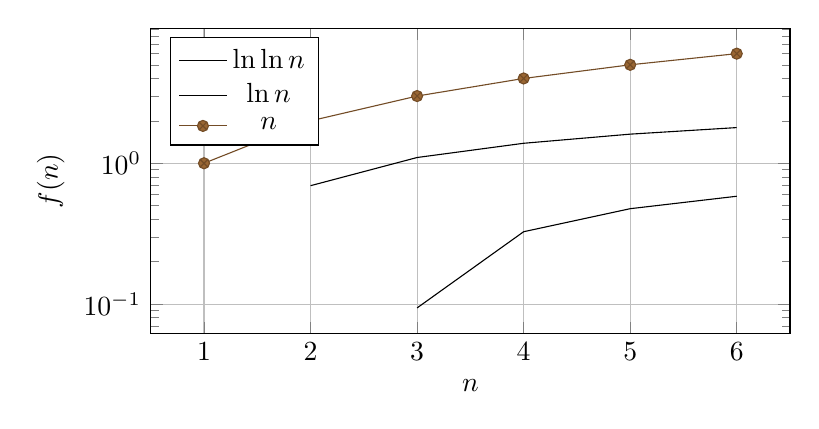
\begin{tikzpicture}
  \begin{axis}[
    width=0.8\textwidth, height=0.45\textwidth,
    xlabel={$n$}, ylabel={$f(n)$}, ymode=log,
    grid=major, legend pos=north west
  ]
  \addplot [domain=2:6, samples=5, mark=none] {ln(ln(x))};
  \addlegendentry{$\ln\ln n$}
  
  \addplot [domain=1:6, samples=6, mark=none] {ln(x)};
  \addlegendentry{$\ln n$}
  
    \addplot coordinates {(1,1) (2,2) (3,3) (4,4) (5,5) (6,6)};
      \addlegendentry{$n$}
  \end{axis}
\end{tikzpicture}
\end{center}

\subsubsection{Exercise 2}
For \(f,g,h\colon\mathbb N\to\mathbb R_{\ge0}\), prove:
\[
\begin{aligned}
1.\;&f\in O(f),\\
2.\;&O(c\,f)=O(f)\quad(\forall c>0),\\
3.\;&f(n)\le g(n)\text{ eventually}\implies O(f)\subseteq O(g),\\
4.\;&O(f)\subseteq O(g)\implies O(f+h)\subseteq O(g+h),\\
5.\;&h(n)>0\;\forall n,\;O(f)\subseteq O(g)\implies O(f\,h)\subseteq O(g\,h).
\end{aligned}
\]

\textbf{Proof.}
\begin{enumerate}[label=\arabic*.]
  \item Since \(f(n)\le1\cdot f(n)\), we have \(f\in O(f)\).
  \item If \(u\in O(c\,f)\), then \(u(n)\le C\,(c\,f(n))\), so \(u\in O(f)\); conversely similarly.
  \item If for large \(n\), \(f(n)\le g(n)\) and \(u\in O(f)\), then \(u(n)\le C\,f(n)\le C\,g(n)\).
  \item If \(u\in O(f)\), then \(u(n)+h(n)\le C\,f(n)+h(n)\le C(f(n)+h(n))\).
  \item If \(u\in O(f)\) and \(h(n)>0\), then \(u(n)h(n)\le C\,f(n)\,h(n)\).
\end{enumerate}

\subsubsection{Exercise 3}
Let \(i,j,k,n\in\mathbb N\).  Prove:
\[
\begin{aligned}
1.\;&j\le k\implies O(n^j)\subseteq O(n^k),\\
2.\;&j\le k\implies O(n^j+n^k)\subseteq O(n^k),\\
3.\;&O\Bigl(\sum_{m=0}^k a_m\,n^m\Bigr)=O(n^k),\\
4.\;&O(\log n)\subseteq O(n),\\
5.\;&O(n\log n)\subseteq O(n^2).
\end{aligned}
\]

\textbf{Proof.}
\begin{enumerate}[label=\arabic*.]
  \item If \(j\le k\), then \(n^j\le n^k\) for \(n\ge1\).
  \item For \(n\ge1\), \(n^j+n^k\le2n^k\).
  \item \(\sum_{m=0}^k a_m\,n^m\le(\sum|a_m|)\,n^k\).
  \item For \(n\ge2\), \(\log n\le n\).
  \item For \(n\ge2\), \(n\log n\le n^2\).
\end{enumerate}

\subsubsection{Exercise 4}
Which relationships hold between:
\[
\begin{aligned}
1.\;&O(n)\text{ vs.\ }O(\sqrt n),\\
2.\;&O(n^2)\text{ vs.\ }O(2^n),\\
3.\;&O(\log n)\text{ vs.\ }O((\log n)^2),\\
4.\;&O(2^n)\text{ vs.\ }O(3^n),\\
5.\;&O(\log_2n)\text{ vs.\ }O(\log_3n).
\end{aligned}
\]
\textbf{Answer.}
\begin{enumerate}[label=\arabic*.]
  \item \(\sqrt n\le n\implies O(\sqrt n)\subsetneq O(n)\).
  \item \(n^2=o(2^n)\implies O(n^2)\subsetneq O(2^n)\).
  \item Eventually \((\log n)^2\ge\log n\implies O(\log n)\subseteq O((\log n)^2)\).
  \item \(2^n\le3^n\implies O(2^n)\subsetneq O(3^n)\).
  \item \(\log_2n=\tfrac{\log_3n}{\log_32}\implies O(\log_2n)=O(\log_3n)\).
\end{enumerate}

\subsubsection{Exercise 5}
Classic sorting comparisons:
\[
\text{bubble sort vs.\ insertion sort},\quad
\text{insertion sort vs.\ merge sort},\quad
\text{merge sort vs.\ quick sort}.
\]
\textbf{Discussion.}
\begin{itemize}
  \item \textbf{Bubble vs.\ Insertion:} Both worst-case \(O(n^2)\), but insertion sort is \(O(n)\) on nearly-sorted input.
  \item \textbf{Insertion vs.\ Merge:} Insertion sort worst-case \(O(n^2)\), merge sort always \(O(n\log n)\), so merge scales better.
  \item \textbf{Merge vs.\ Quick:} Merge sort is \(O(n\log n)\) always; quick sort is \(O(n\log n)\) average, \(O(n^2)\) worst, but faster in practice due to lower constants and in-place partitioning.
\end{itemize}

\subsection{Conclusion}
We’ve surveyed P vs.\ NP, NP-completeness via SAT, practiced ordering and relating functions by asymptotic growth, and applied these insights to sorting algorithms. The included plots illustrate constant-factor and growth-rate comparisons without overwhelming the presentation.

\textbf{Question:} What’s the fastest known quantum sorting algorithm in the query (comparison) model, and how close is it to being practical?


\begin{thebibliography}{9}
\bibitem{hopcroft} Hopcroft, J. E., Motwani, R., Ullman, J. D. \textit{Introduction to Automata Theory, Languages, and Computation}. Pearson, 2007.
\end{thebibliography}

\end{document}
